% =====================================================================
%  FADO architecture -- vector figure (TikZ, standalone PDF)
%  Laid out at the IEEE two-column text width (~18 cm) and included at
%  natural size, so all text is >= 8 pt Times (IEEE template rule).
%  Grey = inherited from Aranyani; blue = adaptive fairness constraint;
%  orange = drift detection and response.
%  Build:  pdflatex fado_architecture.tex
% =====================================================================
\documentclass[tikz,border=1pt]{standalone}
\usepackage{newtxtext,newtxmath}
\usepackage{amsmath}
\usetikzlibrary{positioning,arrows.meta,calc}

\definecolor{ink}{HTML}{1F2328}
\definecolor{muted}{HTML}{57606A}
\definecolor{inhLine}{HTML}{8C959F}
\definecolor{inhFill}{HTML}{FFFFFF}
\definecolor{inhBand}{HTML}{EEF1F4}
\definecolor{conLine}{HTML}{1F5FBF}
\definecolor{conFill}{HTML}{FFFFFF}
\definecolor{conBand}{HTML}{E9F1FC}
\definecolor{drfLine}{HTML}{C2560E}
\definecolor{drfFill}{HTML}{FFFFFF}
\definecolor{drfBand}{HTML}{FDF1E7}

\begin{document}
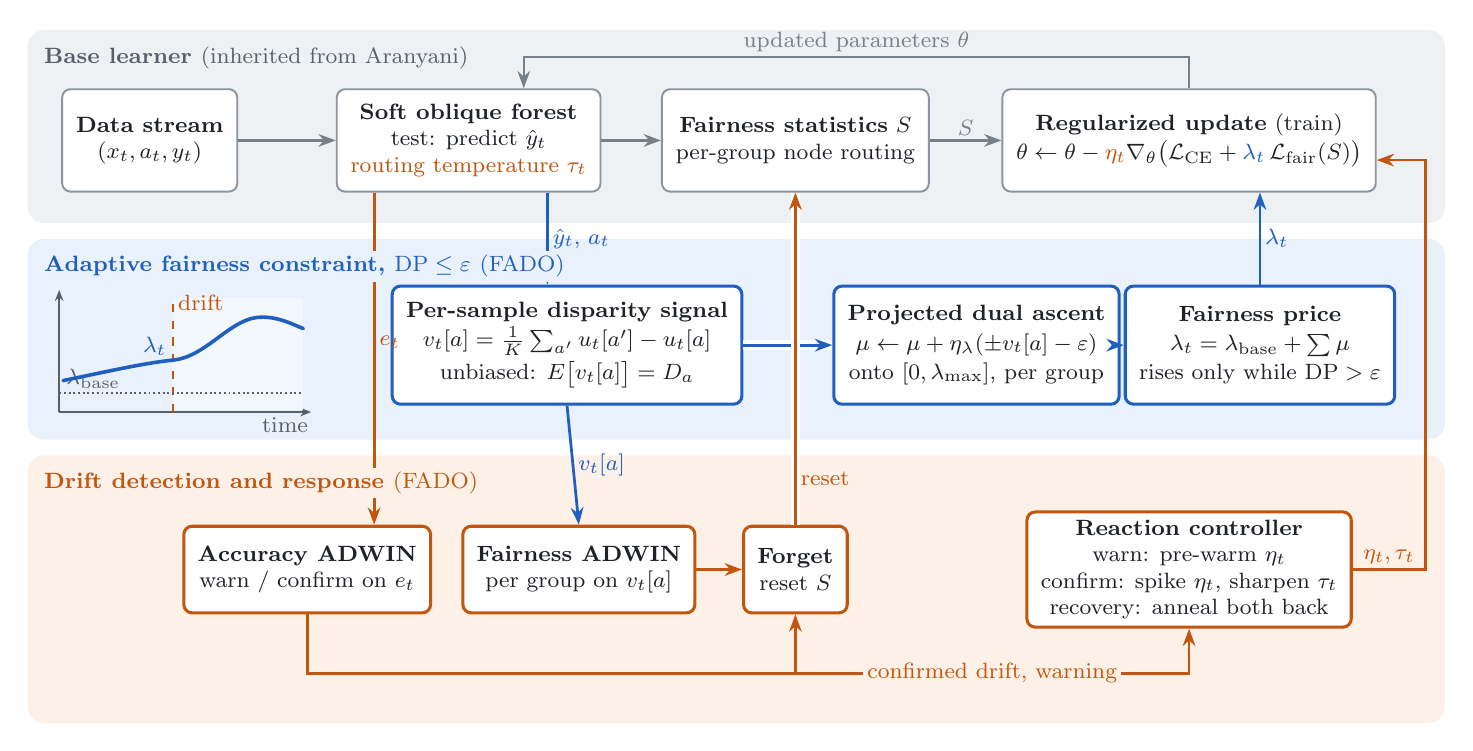
\begin{tikzpicture}[
  font=\footnotesize\color{ink},
  >={Stealth[length=2.2mm,width=1.6mm]},
  box/.style={draw, rounded corners=3pt, align=center, inner xsep=5pt, inner ysep=3pt},
  inh/.style={box, draw=inhLine, fill=inhFill, line width=0.7pt, minimum height=13mm},
  con/.style={box, draw=conLine, fill=conFill, line width=1.1pt, minimum height=15mm},
  drf/.style={box, draw=drfLine, fill=drfFill, line width=1.1pt, minimum height=11mm},
  band/.style={rounded corners=6pt},
  bandlabel/.style={font=\footnotesize\bfseries, anchor=north west, inner sep=0pt},
  flow/.style={->, line width=0.8pt, inhLine!85!black},
  cflow/.style={->, line width=1.0pt, conLine},
  dflow/.style={->, line width=1.0pt, drfLine},
  lbl/.style={font=\footnotesize, inner sep=1.5pt},
  halo/.style={preaction={draw=white, line width=3.4pt, -}},
]

% ------------------------------------------------------------------ bands
\fill[band, inhBand] (0,4.95) rectangle (18,7.4);
\fill[band, conBand] (0,2.2)  rectangle (18,4.75);
\fill[band, drfBand] (0,-1.4) rectangle (18,2.0);

% ------------------------------------------------------------------ base learner (inherited)
\node[inh] (in)     at (1.55,6.0)  {\textbf{Data stream}\\$(x_t,a_t,y_t)$};
\node[inh] (forest) at (5.6,6.0)   {\textbf{Soft oblique forest}\\test: predict $\hat y_t$\\{\color{drfLine}routing temperature $\tau_t$}};
\node[inh] (stats)  at (9.75,6.0)  {\textbf{Fairness statistics} $S$\\per-group node routing};
\node[inh] (update) at (14.75,6.0) {\textbf{Regularized update} (train)\\[1pt]
  $\theta\leftarrow\theta-{\color{drfLine}\eta_t}\nabla_\theta\big(\mathcal{L}_{\mathrm{CE}}+{\color{conLine}\lambda_t}\,\mathcal{L}_{\mathrm{fair}}(S)\big)$};

\draw[flow] (in) -- (forest);
\draw[flow] (forest) -- (stats);
\draw[flow] (stats) -- node[lbl, above]{$S$} (update);
\draw[flow] (update.north) -- ++(0,0.4) -| node[lbl, pos=0.25, above]{updated parameters $\theta$} ([xshift=7mm]forest.north);

% ------------------------------------------------------------------ adaptive fairness constraint (novel)
\node[con] (ht)    at (6.85,3.4)  {\textbf{Per-sample disparity signal}\\[1pt]
  $v_t[a]=\tfrac{1}{K}\sum_{a'}u_t[a']-u_t[a]$\\[1pt] unbiased: $\mathbb{E}\big[v_t[a]\big]=D_a$};
\node[con] (dual)  at (12.05,3.4) {\textbf{Projected dual ascent}\\[1pt]
  $\mu\leftarrow\mu+\eta_\lambda(\pm v_t[a]-\varepsilon)$\\[1pt] onto $[0,\lambda_{\max}]$, per group};
\node[con] (price) at (15.65,3.4) {\textbf{Fairness price}\\[1pt]
  $\lambda_t=\lambda_{\mathrm{base}}+\textstyle\sum\mu$\\[1pt] rises only while $\mathrm{DP}>\varepsilon$};

% inset: the price reacts to a drift (vector sketch)
\begin{scope}[shift={(0.4,2.55)}]
  \draw[muted, line width=0.5pt, ->, >={Stealth[length=1.4mm,width=1.1mm]}] (0,0) -- (3.2,0);
  \draw[muted, line width=0.5pt, ->, >={Stealth[length=1.4mm,width=1.1mm]}] (0,0) -- (0,1.55);
  \fill[conBand!60!white] (1.45,0.02) rectangle (3.1,1.45);
  \draw[drfLine, dashed, line width=0.7pt] (1.45,0) -- (1.45,1.45);
  \node[font=\footnotesize, text=drfLine, anchor=south west, inner sep=1pt] at (1.47,1.25) {drift};
  \draw[muted, densely dotted, line width=0.7pt] (0,0.24) -- (3.1,0.24);
  \node[font=\footnotesize, text=muted, anchor=south west, inner sep=1pt] at (0.05,0.26) {$\lambda_{\mathrm{base}}$};
  \draw[conLine, line width=1.3pt, line cap=round]
    (0.05,0.4) .. controls (0.55,0.5) and (1.05,0.62) .. (1.45,0.66)
    .. controls (1.85,0.7) and (2.15,1.15) .. (2.5,1.2)
    .. controls (2.75,1.23) and (2.95,1.12) .. (3.1,1.06);
  \node[font=\footnotesize, text=conLine, anchor=south east, inner sep=1pt] at (1.4,0.68) {$\lambda_t$};
  \node[font=\footnotesize, text=muted, anchor=north east, inner sep=1pt] at (3.2,-0.03) {time};
\end{scope}

\draw[cflow] ([xshift=10mm]forest.south) -- node[lbl, right]{$\hat y_t,\,a_t$} ([xshift=10mm]forest.south |- ht.north);
\draw[cflow, halo] (ht) -- (dual);
\draw[cflow] (dual) -- (price);
\draw[cflow] (price.north) -- node[lbl, right]{$\lambda_t$} (price.north |- update.south);

% ------------------------------------------------------------------ drift detection and response (novel)
\node[drf] (accmon)  at (3.55,0.55)  {\textbf{Accuracy ADWIN}\\warn / confirm on $e_t$};
\node[drf] (fairmon) at (7.0,0.55)   {\textbf{Fairness ADWIN}\\per group on $v_t[a]$};
\node[drf] (reset)   at (9.75,0.55)  {\textbf{Forget}\\reset $S$};
\node[drf] (react)   at (14.75,0.55) {\textbf{Reaction controller}\\
  warn: pre-warm $\eta_t$\\confirm: spike $\eta_t$, sharpen $\tau_t$\\recovery: anneal both back};

% error stream: forest -> accuracy monitor (left channel, clear of the inset)
\draw[dflow] ([xshift=-12mm]forest.south) -- node[lbl, right, pos=0.45]{$e_t$} ([xshift=-12mm]forest.south |- accmon.north);
% per-sample signal -> fairness monitor
\draw[cflow] (ht.south) -- node[lbl, right]{$v_t[a]$} (fairmon.north);
% detections
\draw[dflow] (fairmon) -- (reset);
\draw[dflow] (accmon.south) -- ++(0,-0.75) coordinate (rail) -| (react.south);
\draw[dflow] (reset.south |- rail) -- (reset.south);
\node[lbl, text=drfLine, fill=drfBand] at ($(reset.south |- rail)!0.5!(react.south |- rail)$) {confirmed drift, warning};
% forgetting clears the statistics (vertical channel through the constraint band)
\draw[dflow, halo] (reset.north) -- node[lbl, right, pos=0.14, text=drfLine]{reset} (stats.south);
% reaction acts on learning rate and routing temperature (right margin)
\draw[dflow] (react.east) -- node[lbl, above, text=drfLine]{$\eta_t,\tau_t$} (17.75,0.55) |- ([yshift=-2.5mm]update.east);

% ------------------------------------------------------------------ band labels (drawn last, over the arrows)
\node[bandlabel, text=muted, fill=inhBand, inner sep=1.5pt]   at (0.15,7.25) {Base learner \textnormal{(inherited from Aranyani)}};
\node[bandlabel, text=conLine, fill=conBand, inner sep=1.5pt] at (0.15,4.6)  {Adaptive fairness constraint, $\mathrm{DP}\le\varepsilon$ \textnormal{(FADO)}};
\node[bandlabel, text=drfLine, fill=drfBand, inner sep=1.5pt] at (0.15,1.85) {Drift detection and response \textnormal{(FADO)}};

\end{tikzpicture}
\end{document}
